\chapter{Estado del Arte}\label{chapter:state-of-the-art}

Este capítulo proporciona una introducción a los campos y los trabajos que
están relacionados con las técnicas utilizadas en esta tesis. Se comienza
introduciendo las ideas básicas de meta-learning~
(Sección~\ref{section:metalearning}), definiendo el problema que este campo
resuelve, explicando la estructura de un sistema de meta-learning y varias de
sus aplicaciones. El objetivo fundamental de este trabajo es añadir componentes
de meta-learning a un sistema de Automated Machine Learning~(AutoML), así que
este campo es introducido~(Sección~\ref{section:AutoML}). Se presentan
diferentes formulaciones teóricas del problema de AutoML y se describen los
componentes fundamentales de un proceso de AutoML, así como ejemplos de
sistemas para cada uno de los enfoques existentes. El área de interés de esta
investigación es la aplicación de meta-learning para la selección de modelos,
en concreto, su utilización para añadir conocimiento en sistemas AutoML, por
lo que varias técnicas para la solución de este problema son estudiadas
(Sección~\ref{section:meta-with-AutoML}).

\section{Meta-Learning}\label{section:metalearning}

El término meta-learning ocurrió por primera vez en el área de psicología
educacional. Uno de los investigadores más citados en este campo, John Biggs,
describió meta-learning ``como ser consciente y tomar el control del
conocimiento de uno''~\brackcite{biggs1985role}. Por lo tanto, meta-learning
es visto como un entendimiento y adaptación del aprendizaje en sí en un nivel
más alto que simplemente adquirir conocimiento de una materia. Una persona
consciente y capaz de meta-learning es capaz de evaluar su enfoque de
aprendizaje de acuerdo a los requerimientos de una tarea en específico.

Meta-learning usada en el contexto de aprendizaje automático tiene muchas
similitudes a esta descripción. El conocimiento de una materia se traduce en
\textit{base-learning}, donde la experiencia es acumulada para una tarea en
específico. Meta-learning empieza en un nivel mayor y se encarga de acumular
experiencia sobre varias aplicaciones de un sistema de
aprendizaje~\brackcite{hospedales2021metalearning}.

Debido al creciente poder de computación y gran disponibilidad de conjuntos de
datos en los últimos 20 años, la investigación de aprendizaje automático
enfrentó un creciente número de algoritmos disponibles, incluyendo multitudes
de parametrizaciones, enfoques de pre-procesamiento y pos-procesamiento, así
como una gran variedad de aplicaciones~\brackcite{lemke2013metalearning}.
Promoviendo un mejor entendimiento del aprendizaje automático en sí,
meta-learning puede ser de una ayuda invaluable, evitando procedimientos
extensivos de prueba y error para la selección de algoritmos. Además, puede
permitir entender mejor que hace a un determinado algoritmo desempeñarse bien
en un determinado problema. En esta sección se estudia la definición de
meta-learning, la estructura de un sistema de meta-learning y algunas de sus
aplicaciones.

\subsection{Definición}\label{subsec:meta-definition}

La primera definición de meta-learning en el campo de aprendizaje automático
fue dado por J\"ugen Schmidhuber en 1987, el cual lo considera la interacción
entre agente y el ambiente impulsando la superación personal en el agente.
Meta-learning es mejor entendido comúnmente como ``aprendiendo a aprender'',
lo cual se refiere al proceso de mejorar un algoritmo de aprendizaje a través
de múltiples episodios de aprendizaje. En contraste, el aprendizaje automático
convencional mejora las predicciones del modelo sobre múltiples instancias de
datos. Durante el \textit{base-learning} o aprendizaje base, un algoritmo de
aprendizaje interior~(o inferior/base) resuelve una tarea como clasificación
de imágenes, definida por un conjunto de datos y un objetivo. Durante
\emph{meta-learning}, un algoritmo externo~(o superior/meta) actualiza el
algoritmo interior de tal manera que el modelo que aprende mejora un objetivo
externo. Los episodios de aprendizaje de la tarea base pueden ser vistos como
una forma de proveer las instancias necesitadas por el algoritmo externo para
aprender el algoritmo de aprendizaje base~\brackcite{hospedales2021metalearning}.

Meta-learning difiere de \textit{base-learning} en el alcance del nivel de
adaptación. Mientras que el aprendizaje en un nivel base está enfocado en
acumular experiencia en una tarea específica, el aprendizaje en meta-learning
tiene el objetivo de acumular experiencia en el rendimiento de múltiples
aplicaciones de un sistema de aprendizaje. De esta forma, muchos algoritmos
convencionales tales como la búsqueda aleatoria de hiperparámetros mediante
validación cruzada podrían caer en la definición de meta-learning. La
característica destacada del \emph{meta-learning} contemporáneo es un
meta-objetivo explícitamente definido, y una optimización de extremo a extremo
del algoritmo interior con respecto a este objetivo.

\subsection{Campos relacionados}\label{subsec:meta-related-fields}

Aquí se posiciona meta-learning contra áreas relacionadas cuya relación con
meta-learning es a menudo una fuente de confusión
\brackcite{hospedales2021metalearning}:

\begin{description}
	\item[Transfer Learning (TL):] TL usa experiencia pasada de una tarea
    fuente para mejorar el aprendizaje~(la velocidad, la eficiencia de los
    datos, la precisión) de una tarea destino. TL se refiere a esta área de
    problemas como familia de soluciones, y para su solución hace uso de la
    transferencia de parámetros, más el ajuste opcional de los mismos. En
    contraste, meta-learning se refiere al paradigma que puede ser utilizado
    para mejorar TL, así como otros problemas. En TL el modelo final es
    extraído por aprendizaje simple en la tarea fuente sin el uso de un
    meta-objetivo. En meta-learning, el modelo final estaría definido por la
    optimización externa que evalúa el beneficio del modelo cuando aprende una
    nueva tarea.
	
	\item[Aprendizaje multi-tarea (MTL):] intenta aprender en conjunto algunas
    tareas relacionadas para beneficiarse de la regularización debido al
    intercambio de parámetros y la diversidad de la representación compartida
    resultante. Como TL, MTL convencional es una optimización de un solo nivel
    sin un meta-objetivo. Además, el propósito de MTL es el de aprender de una
    cantidad fija de tareas conocidas, mientras que el objetivo de
    meta-learning es a menudo aprender de tareas futuras no vistas.
	 
	\item[Optimización de Hiperparámetros (HPO):] está dentro de las
    consideraciones de meta-learning, en el sentido de que hiperparámetros como
    la tasa de aprendizaje o la fuerza de regularización describen
    ``cómo aprender''. Aquí se suelen incluir tareas de HPO que definen un
    meta-objetivo que es entrenado de extremo a extremo con redes neuronales,
    tales como el aprendizaje de hiperparámetros basados en gradientes y la
    búsqueda de arquitectura neuronal. Pero excluyen otros enfoques como
    búsqueda aleatoria y optimización bayesiana, las cuales raramente están
    consideradas como meta-learning~\brackcite{hospedales2021metalearning}.
	
	\item[AutoML:] AutoML es más bien un espectro amplio de enfoques con el
    objetivo de automatizar partes del proceso de aprendizaje automático que
    son típicamente manuales, tales como la preparación de los datos, la
    selección de algoritmos, ajuste de hiperparámetros, y búsqueda de
    arquitecturas. AutoML a menudo utiliza numerosas heurísticas afuera del
    alcance de meta-learning, y se usa en tareas como limpieza de datos, que
    son menos importantes en meta-learning. Sin embargo, AutoML a veces
    utiliza optimizaciones de extremo a extremo de un meta-objetivo, así que
    meta-learning puede ser visto como una especialización de AutoML. AutoML
    a menudo usa técnicas de meta-learning para inicializar su proceso de
    optimización y ganar experiencia de experimentaciones pasadas.
\end{description}

\subsection{Estructura de un Sistema de Meta-Learning}

Un sistema de meta-learning está compuesto esencialmente por dos partes. Una
parte tiene la tarea de adquirir meta-conocimiento de sistemas de aprendizaje
automático. La otra parte tiene el objetivo de aplicar este meta-conocimiento
a nuevos problemas con el objetivo de identificar un algoritmo o técnica de
aprendizaje óptimo.

\subsubsection{Adquisición de Meta-Conocimiento} 

Hay dos modos naturales en los cuales el meta-conocimiento puede ser adquirido.
Una posibilidad es depender de conocimiento experto y otra posibilidad es usar
un procedimiento automático. 

La obtención de meta-conocimiento a través del conocimiento experto se realiza
en la forma de reglas que coinciden con las características de dominio~
(conjunto de datos) y con algoritmos de aprendizaje automático. Estas reglas
pueden ser hechas a mano, teniendo en cuenta resultados teóricos, el
conocimiento humano y evidencia empírica. Sin embargo, este método tiene serias
desventajas: el conjunto de reglas resultantes probablemente esté incompleto y
el mantenimiento del conjunto de reglas a medida que nuevos algoritmos se
vuelven disponibles es problemático. Como resultado, la mayoría de la
investigación se ha enfocado en métodos automáticos
~\brackcite{bradzil2017metalearning}.
	
Para la automatización de la adquisición de conocimiento es necesario un
conjunto de problemas y un conjunto de algoritmos de aprendizaje automático
que queremos considerar. Entonces se necesita definir un método experimental
que determine con cuáles alternativas deberíamos experimentar y en qué orden.
Por ejemplo, dado un conjunto de datos~(con ciertas características) y
ciertos algoritmos de aprendizaje automático, se producen resultados de
rendimiento para cada uno de estos algoritmos a través de un método de
evaluación~(como validación cruzada). Los resultados y la estructura de los
algoritmos aplicados, junto con la caracterización de los conjuntos de datos,
representan un pedazo de información que es guardado en una base de
meta-conocimiento. El proceso es entonces repetido para otras combinaciones de
conjuntos de datos y algoritmos. 
En la Figura~\ref{fig:adquisition} se muestra cómo se realiza el proceso de
adquisición del meta-conocimiento.

\begin{figure}[H]
    \centering
    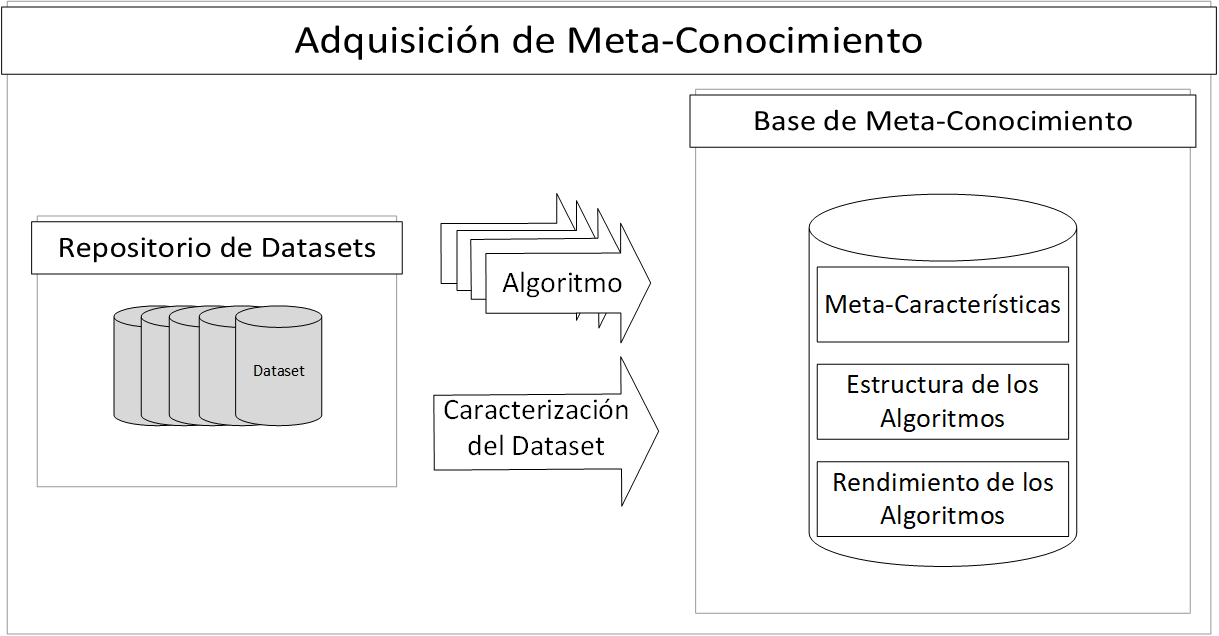
\includegraphics[scale=.5]{Figures/adquisition.png}
    \caption{Proceso de adquisición de meta-conocimiento. }
    \label{fig:adquisition}
\end{figure}

\subsubsection{Aplicación de Meta-Conocimiento}

En un sistema de meta-learning la aplicación de meta-conocimiento puede ser
usada para ayudar a seleccionar o adaptar algoritmos de aprendizaje automático.
Por ejemplo, se puede considerar nuestro problema de la selección de algoritmos
de aprendizaje automático dado un determinado conjunto de algoritmos. Este
puede ser visto como un problema de búsqueda, donde el espacio de búsqueda
incluye los algoritmos de aprendizaje automático individuales y el objetivo es
identificar el mejor algoritmo. Este proceso puede ser dividido en dos fases
separadas. La Figura~\ref{fig:application} muestra un diagrama de como ocurre
este proceso.

En la primera fase~(Figura~\ref{fig:application} a) el objetivo es identificar
un subconjunto adecuado de algoritmos de aprendizaje automático basados en un
conjunto de datos de entrada. El método de selección empleado en ese proceso se basa en
el meta-conocimiento. Dado un nuevo conjunto de datos sus meta-características son
extraídas y estas son analizadas para extraer de la base de meta-conocimiento
los conjunto de datoss similares. Por lo general, el resultado de esta fase es
representado en la forma de un subconjunto rankeado de algoritmos de
aprendizaje automático.

La segunda fase~(Figura~\ref{fig:application} b) tiene el objetivo de buscar a
través del espacio reducido. Cada opción es evaluada empleando una métrica de
rendimiento determinado~(por ejemplo, \textit{accuracy}). Usualmente, la
validación cruzada es usada para identificar el mejor algoritmo de aprendizaje.
Es necesario notar que el meta-conocimiento no elimina completamente la
necesidad del proceso de búsqueda, sino que proporciona una búsqueda más
efectiva. La efectividad de la búsqueda depende de la calidad del
meta-conocimiento~\brackcite{bradzil2017metalearning}.


\begin{figure}[H]
	\centering
	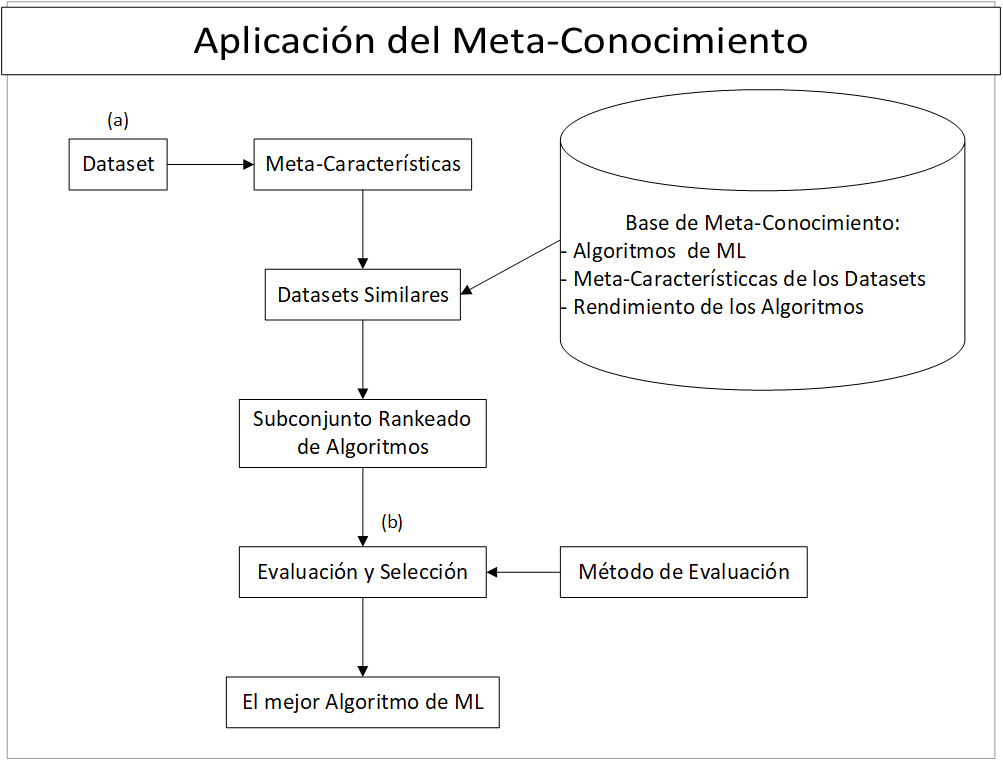
\includegraphics[scale=.5]{Figures/application.png}
	\caption{Proceso de aplicación de meta-conocimiento.}
	\label{fig:application}
\end{figure}

\subsection{Aplicaciones de Meta-Learning}\label{subsec:mtl_aplications}

Meta-learning puede ser empleada en una variedad de configuraciones, con cierto
desacuerdo en la literatura sobre lo que constituye exactamente un problema de
meta-learning. Meta-learning es extremadamente útil en los casos donde es
requerido un modelo de aprendizaje automático y hay poca cantidad de datos,
ya que el modelo contiene muchos parámetros que no pueden ser estimados
precisamente con pocos datos. Algunas de las aplicaciones comunes son en la
investigación robótica, donde se espera que los robots tengan un mayor nivel
de autonomía en IA, en el descubrimiento de drogas para manejar los datos de 
altas dimensiones con un tamaño de muestra pequeño y en la traducción de
lenguajes raramente usados~\brackcite{peng2020comprehensive}.

Meta-learning constituye una solución factible para los problemas donde una
definición específica de ``tarea'' y ``etiqueta'' puede ser claramente
distinguida. Un sistema de meta-learning es flexible y puede ser
integrado convenientemente con la mayoría de los algoritmos de aprendizaje
automático para proporcionar soluciones factibles~\brackcite{peng2020comprehensive}.
Para las tareas que son computacionalmente costosas, meta-learning presenta la
opción de agregación o adaptación de los resultados anteriores para salvar
recursos computacionales.

\section{AutoML}\label{section:AutoML}

\textit{Automated Machine Learning}~(AutoML) o Aprendizaje de Máquinas
Automático es el campo que se enfoca en los métodos que tienen el objetivo de
automatizar diferentes etapas del proceso de aprendizaje automático. Como su
nombre indica, AutoML es la intersección de dos campos: automatización y ML.
Las soluciones de AutoML están recibiendo incrementalmente más atención tanto
por la comunidad de ML como por los usuarios por las grandes cantidades de
datos disponibles en todas partes y la falta de expertos de aprendizaje
automático que puedan supervisar/asesorar el desarrollo de sistemas basados en
ML~\brackcite{hutter2019autmlbook}.

La diferencia entre el aprendizaje automático clásico y AutoML es que en el
primero, los humanos están grandemente involucrados en la configuración de las
herramientas de aprendizaje realizando ingeniería de características, selección
y evaluación de modelos. Como resultado, los humanos realizan la mayor parte
del trabajo en las prácticas del aprendizaje automático. Sin embargo, en
AutoML, todo esto puede ser hecho con programas de forma automática.

La comunidad de AutoML se ha centrado en resolver varias partes de un flujo de
trabajo de aprendizaje automático estándar. Algunos ejemplos de estas partes o
subtareas que son aplicadas en AutoML son:

\begin{description}
	\item[\textit{Automated Data Preparation} o Preparación Automática de
    Datos:] el flujo de trabajo de la preparación de datos está compuesto por 
    3 componentes: colección de datos, limpieza de datos e incremento de datos.
    La colección de datos es un paso necesario para construir un nuevo conjunto
    de datos o extender el conjunto de datos existente. El proceso de limpieza
    de datos es usado para filtrar los datos con ruido para que el
    entrenamiento del modelo no sea comprometido. El incremento de datos tiene
    un rol importante en mejorar la robustez del modelo y mejorar su
    rendimiento. Este paso es uno de los que más difícilmente son
    automatizados~\brackcite{he2021automl}.
	
	\item[\textit{Automated Feature Engineering} o Ingeniería Automática de
    Características:] el objetivo de ingeniería de características es construir
    más características para mejorar el rendimiento de aprendizaje cuando las
    características no son lo suficientemente informativas. Para esto se diseña
    un modelo que aprende de las características de entrada para construir
    nuevas características, con las cuales el algoritmo de aprendizaje
    automático obtiene un mejor rendimiento. Con la automatización de esta
    tarea se elimina parte de la asistencia humana para construir
    automáticamente nuevas características~\brackcite{he2021automl}.
	
	\item [\textit{Neural Architecture Search} (NAS) o Búsqueda de
    Arquitecturas Neuronales:] el objetivo de NAS es encontrar una arquitectura
    de redes neuronales profundas con buen rendimiento en un conjunto de datos
    determinado. NAS ha sido usado para diseñar redes que están a la par o
    tienen mejores resultados que arquitecturas diseñados a man
    ~\brackcite{zoph2017learning, witsuba2019nas}. Aunque es una práctica común
    optimizar la arquitectura y las configuraciones de los hiperparámetros en
    secuencia, existe evidencia reciente de que deberían ser optimizadas en
    conjunto \brackcite{bischl2021hyperparameter}.
\end{description}

Sin embargo, los estudios recientes de AutoML buscan automatizar el flujo de
algoritmos de aprendizaje automático entero~\brackcite{fuerer2015efficient,
paszke2019pytorch}. Un flujo de algoritmos es una forma de codificar y
automatizar el flujo de trabajo necesario para producir un modelo de
aprendizaje automático. Los flujos de algoritmos de aprendizaje automático
constan de varios pasos secuenciales que realizan desde la extracción de datos
y el preprocesamiento hasta el entrenamiento y la implementación del modelo
~\brackcite{web-mlpipe}.

\subsection{Definición del problema}\label{subsec:automl_problem_definition}

Dos problemas importantes en AutoML son que ningún algoritmo de ML obtiene los
mejores resultados en todos los conjunto de datoss, también conocido como
\textit{No Free Lunch Problem}~\brackcite{wolpert1995no}, y que algunos métodos de
aprendizaje automático dependen crucialmente de la optimización de
hiperparámetros. Para la resolución de estos problemas AutoML se apoya de dos
áreas o subtareas que constituyen su base: la selección de modelos~
(\textit{Model Selection}, MS)~\brackcite{thornton2013auto} y la optimización de
hiperparámetros (\textit{Hyperparameter Optimization}, HPO)
~\brackcite{fuerer2019hyperparameter}. La combinación de estas áreas se refiere al
problema de AutoML como un problema de selección combinada de modelos y
optimización de hiperparámetros~(\textit{Combined Algorithm Selection and
Hyperparameter Optimization}, CASH)~\brackcite{thornton2013auto}.

\subsubsection{Selección de Modelos}

El objetivo de la selección de modelos es encontrar un algoritmo de aprendizaje
automático adecuado para un conjunto de datos determinado. Hay muchos aspectos de los
cuales un científico de datos se preocupa en la selección de algoritmos, tales
como la complejidad computacional, diferencias en el tiempo de entrenamiento y
si el algoritmo permite una entrada no lineal, y es útil considerar estos
aspectos en la automatización. Para realizar esta tarea un sistema AutoML
realiza una búsqueda sobre un conjunto de algoritmos disponibles, con el
objetivo de determinar cuáles de ellos pertenecen al flujo óptimo de un
problema determinado~\brackcite{li2021automl}.

\subsubsection{Optimización de Hiperparámetros}

Los algoritmos de aprendizaje automático son altamente configurables por sus
hiperparámetros~(HP). Estos últimos a menudo influencian substancialmente el
comportamiento y la velocidad del algoritmo y tienen que ser seleccionados con
cuidado con el objetivo de alcanzar un rendimiento óptimo. Tanto para expertos
como para no expertos, ajustar los hiperparámetros para optimizar el
rendimiento del modelo puede ser una tarea difícil y tediosa, a menudo es
bastante costosa y propensa a errores, especialmente cuando son seleccionados
en un proceso de prueba y error. Los algoritmos de optimización de
hiperparámetros~(HPO) identifican automáticamente una configuración de
hiperparámetros~(HPC) buena para un algoritmo de ML, reduciendo así el esfuerzo
humano. Por lo tanto, una de las tareas fundamentales de AutoML es ajustarlos
para optimizar el rendimiento de los algoritmos de ML~\brackcite{li2021automl}.

\section{Meta-Learning en AutoML}\label{section:meta-with-AutoML}

La principal área de investigación de meta-learning estudiada en este trabajo
es la selección de algoritmos, la cual ha recibido una considerable cantidad
de investigación. En el caso especial de meta-learning, el aspecto de interés
es la relación entre las características de los datos y el rendimiento del
algoritmo, con el objetivo final de predecir un algoritmo o un conjunto de
algoritmos adecuado para un problema específico. Como motivación está el hecho
de que es inviable examinar todas las posibles alternativas de algoritmos en un
procedimiento de prueba y error. La aplicación de meta-learning en este campo
puede, por lo tanto, ser útil tanto para proveer una recomendación para un
usuario final como de paso preliminar para recomendar algoritmos a soluciones
más costosas computacionalmente, como los algoritmos de optimización usados en
herramientas de AutoML. 

El desafío en meta-learning para la selección de modelos es aprender de
experiencias pasadas de una forma sistemática e impulsada por los datos.
Primero, es necesario extraer los meta-datos que describen las tareas de
aprendizaje anteriores y los modelos previamente aprendidos. Estos meta-datos
comprenden las configuraciones exactas de los algoritmos empleados para
entrenar los modelos, incluyendo:

\begin{itemize}
	\item Las configuraciones de los hiperparámetros, composiciones de los
    flujos de algoritmos y/o arquitecturas de redes neuronales.
	\item Las evaluaciones del modelo resultante, tales como la precisión y el
    tiempo de entrenamiento.
	\item Propiedades medibles de la tarea en sí, que son extraídas de los
    conjuntos de datos, también conocidas como meta-características.
\end{itemize}

Luego es necesario aprender de estos meta-datos previos, para extraer y
transferir conocimiento de la búsqueda de los modelos óptimos para nuevas
tareas. El resto de esta sección presenta una visión general de diferentes
enfoques de meta-learning para hacer esto efectivamente. Además, se muestran
ejemplos de cómo estos enfoques han sido utilizados como paso preliminar en
varias herramientas de AutoML.

\subsection{Meta-Características}

Cómo extraer información adecuada para caracterizar tareas específicas es una
de las preguntas fundamentales en meta-learning. Investigadores han intentado
contestar esta pregunta observando las características de los conjuntos de datos
que afectan el rendimiento de los algoritmos~\brackcite{Rivolli2018TowardsRE}. Estas
caracterizaciones son denominadas meta-características y usualmente se
encuentran divididos en cinco grupos. Estos grupos son subconjuntos de medidas
de caracterización \brackcite{bradzil2009metalearning} que comparten similitudes
entre ellas:

\begin{description}
	\item[Simple:] son características que son fácilmente extraídas de los
    datos, son conocidas comúnmente y no requieren recursos computacionales
    significativos. Representan información básica sobre el conjunto de datos.
    Hasta un determinado punto son concebidas para medir la complejidad del
    problema subyacente. Algunas de las caracterizaciones incluidas en este
    grupo son: el número de instancias, el número de atributos, la
    dimensionalidad del conjunto de datos, la proporción de valores faltantes,
    etc. También son llamadas medidas \textit{generales}.
	
	\item[Estadísticas:] son características que capturan las propiedades
    estadísticas de los datos. Estas métricas capturan los indicadores de
    distribución de datos, tales como la media, la desviación estándar,
    la correlación y curtosis. Solo caracterizan los atributos numéricos. Las
    caracterizaciones estadísticas son deterministas y algunas de ellas
    requieren la definición de valores de hiperparámetros.
	
	\item[Teóricas de la información:] son características del campo de teoría
    de la información. Estas medidas están basadas en la entropía, la cual
    captura la cantidad de información en los datos y su complejidad. Ellas
    pueden ser usados para caracterizar los atributos discretos. Además, son
    computadas directamente, libres de hiperparámetros, deterministas y
    robustas. Semánticamente, describen la variedad y la redundancia de los
    atributos utilizados para representar las clases.
	
	\item[Basados en modelos:] son características extraídas de un modelo
    inducido de los datos de entrenamiento. Las características en este grupo
    están caracterizadas por la extracción de información de un modelo de
    aprendizaje de predicción, generalmente, un árbol de decisión. Las medidas
    caracterizan la complejidad de los problemas basados en las hojas, los
    nodos y la forma del árbol. Están diseñadas para caracterizar problemas
    supervisados, todas las medidas son deterministas, robustas y requieren la
    definición de los hiperparámetros que hay en el algoritmo de árboles de
    decisión para inducir el modelo.
	
	\item[\textit{Landmarking}:] son características que usan el rendimiento de
    algoritmos de aprendizaje simples y rápidos para caracterizar los conjunto
    de datoss. Los algoritmos deben tener diferentes sesgos y capturar
    información importante con un costo computacional bajo. Las medidas
    caracterizan problemas supervisados y son indirectamente extraídas.
    Requieren la definición de hiperparámetros: el algoritmo de aprendizaje,
    la medida de evaluación usada para comprobar el rendimiento del modelo y
    el procedimiento empleado para calcularla~(por ejemplo, validación cruzada).
\end{description}

Los primeros tres grupos representan los enfoques más comunes y tradicionales
de las caracterizaciones de los datos. Los últimos dos requieren el uso de
algoritmos de aprendizaje automático, porque extraen la complejidad del modelo
o medidas de rendimiento del mismo, haciéndolos además más complejos.

\section{Conclusión}\label{sec:conclusion}

La democratización de la Inteligencia Artificial es una de las preocupaciones
fundamentales, tanto de la comunidad científica como de los expertos de la
industria. El campo del AutoML se presenta como una alternativa prometedora
para disminuir substancialmente el esfuerzo que conlleva la aplicación de
técnicas de inteligencia artificial, y específicamente de aprendizaje
automático, a problemas concretos. Por otro lado, el campo de meta-learning
aplicado a AutoML permite reusar conocimiento previo para solucionar nuevas
tareas. Este tipo de estrategias ayuda a disminuir el costo de aplicar AutoML,
al relacionar un nuevo conjunto de datos con los mejores flujos obtenidos en
problemas similares previamente resueltos. La habilidad de los sistemas de
computación de guardar virtualmente grandes cantidades de experiencias pasadas
de aprendizaje~(en forma de meta-datos) abre una gran cantidad de oportunidades
de usar esa experiencia en maneras completamente diferentes
~\brackcite{vanschoren2018metalearning}.

Aunque existen varias herramientas de meta-learning que han sido exitosas al
aplicarse a AutoML resolviendo problemas específicos de inteligencia
artificial, estas herramientas son aún demasiado rígidas para ser utilizadas
en problemas prácticos que requieren la combinación de algoritmos y tecnologías
de diferente naturaleza. Por lo tanto, la herramienta de meta-learning creada
tiene el objetivo de abordar una gran variedad de problemas mediante la
selección de meta-características capaces de representarlas. Además, es
necesario el uso de un sistema complementario de AutoML capaz de generar
soluciones eficaces para una amplia gama de tareas y dominios. Por esta razón,
se utiliza de AutoGOAL\brackcite{estevanellhacia}, que destaca por su
capacidad de abordar diferentes dominios combinando de forma transparente
técnicas y herramientas dispares. AutoGOAL usa como método de optimización
\textit{Probabilistic Grammatical Evolution}~\brackcite{estevez2021general}~(PGE),
que no había sido usado anteriormente junto con meta-learning, lo que añade
complejidad a la propuesta. El uso de esta estrategia de meta-learning
permitirá disminuir el costo de aplicar AutoML y generalizar AutoML a dominios
novedosos.
